\documentclass[11pt]{scrartcl}
\usepackage[parfill]{parskip}
\usepackage{graphicx}
\usepackage{booktabs}
\usepackage{tabulary}
\usepackage{float}
\usepackage{hyperref}

\graphicspath{{../images/}}

\title{\textbf{Project Management}}
\subtitle{Final assignment\\
            Release of a FLOSS product by a SME}
\author{Ricardo Garc\'ia Fern\'andez}
\date{\today}

\begin{document}

\maketitle

\vfill

\begin{flushright}
    \copyright  2013 Ricardo Garc\'ia Fern\'andez - ricardogarfe [at] gmail [dot] com.

    This work is licensed under a Creative Commons 3.0 Unported License.
    To view a copy of this license visit:
 
    \url{http://creativecommons.org/licenses/by/3.0/legalcode}.
\end{flushright}

\begin{figure}[h]
    \begin{flushright}	
        
\includegraphics{by}
        \label{fig:by}
    \end{flushright}
\end{figure}

\newpage

\tableofcontents

\newpage

\section{SME Introduction}
\label{sec:sme-introduction}

\par \emph{Code Garden} is our SME. We develop software products using quality patterns. Quality patterns are our main goal, applying Quality patterns to software development as is. plants and the code can not be kept alone, they can grow with life, diverted, or wither in a forgotten place. So plants like the code, need extra care, some gardeners, so they can grow and flourish. 

\par \emph{Technical Debt} is not a monster chasing us in every development sprint is another \emph{ROL} that we accept and we have interaction with it. We need him and he needs us.

\par Thus, we created a software product that helps us to deal with Technical Debt, \textbf{Greenhouse}.

\par \emph{Greenhouse} is our tool to track the progress of the evolution of code quality within a controlled environment. Using quality metrics for each programming language helps us reduce technical debt faster

\begin{quote}
    \begin{center}
    \emph{"we are the code we write"}
    \end{center}
\end{quote}

% section sme-introduction (end)
\section{Publish the project}
\label{sec:publish-project}

\par We want to publish \emph{Greenhouse} as a FLOSS\footnote{Free Libre Open Source Software} project with two Software Licenses.

\par One a FLOSS License and the other a Private License. We chose a \emph{Dual-License} product.

\par Thus we can serve every type of costumers as MySQL business model explained by Elena Blanco\cite{dl-business-model}.

\begin{quotation}
    \emph{For anyone who wants to develop and distribute but does not want to release the source code for their application, MySQL is able to provide a commercial licence. Because MySQL has full ownership of the MySQL code, it is able to tailor its commercial licensing terms to meet the unique requirements of users interested in embedding or bundling MySQL.}
\end{quotation}

\subsection{Dual License}
\label{sub:dual-license}

\par Free Software License and Private, Brief discussion about licenses (your company has heard about some BSD or GPL, but they are not sure!).

\par FLOSS License selected to publish \emph{Greenhouse} is \emph{GPLv3}\footnote{GNU Public License Version 3 - \url{http://www.gnu.org/licenses/gpl-3.0.html}}. This FLOSS License provides all freedoms to the project:

\begin{itemize}
	\item the freedom to use the software for any purpose,
	\item the freedom to change the software to suit your needs,
	\item the freedom to share the software with your friends and neighbors, and
	\item the freedom to share the changes you make.
\end{itemize}

\par The other License is a private License. A private License gives us more flexibility through market niche.

\par Good thing to take in advance using a Private License are:

\begin{itemize}
	\item Avoid possible or unexpected License Violations.
	\item Build a project in your company and be 100\% sure that you are not violation any License under your product.
	\item This License envelops the whole product into a private version.
\end{itemize}

\par This private License gives you the opportunity to deal with \emph{Greenhouse} libraries and include into other projects using full capabilities. This way you can avoid License problems with derivated works and be compatible with other FLOSS Licenses.

\par Brian Behlendorf\cite{brian-behlendorf-business-strategy} explains this model with a success and its weaknesses with the community development:

\begin{quotation}
    \emph{You have to be very careful, though, to make sure that any code volunteered to you by third parties is explicitly available for this non-free branch; you ensure this by either declaring that only you (or people employed by you) will write code for this project, or that (in addition) you'll get explicit clearance from each contributor to take whatever they contribute into a non-free version.}
\end{quotation}

\par We are very concerned about how to interact with the community. Our goal is provide to community the opportunity to develop solutions to our clients for \emph{Greenhouse}.

\begin{quotation}
    \emph{I would claim that if you treat your contributors right, perhaps even offer them money or other compensation for their contributions (it is, after all, helping your commercial bottom line), this model could work.}
\end{quotation}

\par Last quotation is how \emph{Transvirtual}\footnote{\url{http://www.transvirtualsystems.com/}} in Berkeley applied this model to a commercial lightweight Java. Encourage the developers to work and earn money directly with the software they make. We believe in this model to create a community involved around the product: 

\begin{itemize}
	\item The usability of the product.
	\item Tangible incentives as our case the money.
\end{itemize}

\par In this way we will try to solve the dilemma of FLOSS developments that can be converted into proprietary solutions.

\par Therefor, an exchange of knowledge by salaries to the community through an assignment of copyright to Code Garden by using the \emph{GPLv3 License}, they maintain the authoring and earn tangible rewards too.

\par We are the copyright holders of \emph{Greenhouse} and thus , we want to share the maintenability with community knowledge to provide solutions for companies with private Licenses of the product.

\par We want to evolve with the community and spread our developments and remain FLOSS.

% subsection dual-license (end)
% section publish-project (end)
\section{Market niche - Competitors analysis}
\label{sec:market-niche}

\par Code analysis is increasing everyday in software development. SME \& Big Enterprises focus its products near quality. Why ? Because Software Development is measurable, high measurable I could say. Every software is developed guided by patterns through developers and the final product (talking about clients) is released to the client showing its functionality but what happens with all the code developed inside ?

\par The code evolves as the development grows. In a development team is difficult to measure the quality of the product grained.

\par Other sample of the use of measure the quality is when you have to choose between two libraries to implement another service that use the functionality implemented by them. One metric to take care is the code quality that you can apply for them. Using some objective metrics you can retrieve a numeric result that gives you a general idea. Or if you want to add an existing module/library you can choose the one which its result is near to your software, not lesser not higher. It is a way of seeking for a balance in development and knowledge about complexity of a module to import to your product.

\par There are some samples of Analyzing tools but we are to analyze \emph{Code Climate} and \emph{Sonar}.

\subsection{Code climate}
\label{sub:code-climate}

\textbf{Code climate} - \url{https://codeclimate.com/}. Code quality analysis in Ruby Language. But we will not focus on language but with what gives us the tool.

\begin{figure}[H]
\centering
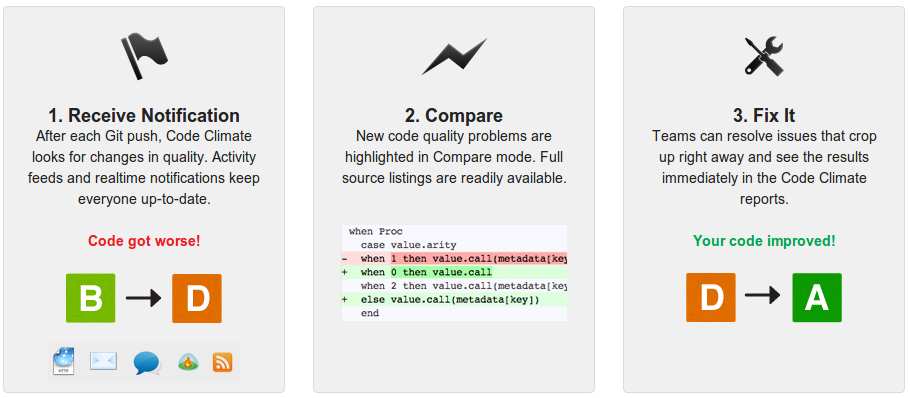
\includegraphics[width=0.7\textwidth]{code-climate.png}
\caption{Code Climate Notifications}
\label{}
\end{figure}

\par This tool gives us interoperability with Software Forges like Github integration. Source Code Management with Git repositories, Code Quality evolution, Notifications, Comparison tools. This tool set is simple but efficient, this is very important. Play with the ease of integration into a forge development offering hosting server, pay and enjoy the product (one click purchase).

\par Includes the main features of services; \emph{PaaS}\footnote{Platform as a Service}, \emph{IaaS}\footnote{Infrastructure as a Service} and \emph{SaaS}\footnote{Software as a Service}. Using \emph{bluebox services} - \url{https://bluebox.net/}: Virtualized Environments on Actual Hardware.

\par We want those services available for every developer and easily result visualization.

\par It's free (gratis) to use for FLOSS projects.

% subsection code-climate (end)

\subsection{Sonar}
\label{sub:sonar}

\textbf{Sonar} - \url{http://www.sonarsource.org/}. Sonar slogan is very clear:

\begin{quote}
    \emph{Put your technical debt under control}
\end{quote}

\par Despite Code Climate, Sonar covers lots of languages and is a FLOSS product. A very good point to consider for the use of this software. Controls and test every corner of your project.

\begin{figure}[H]
\centering
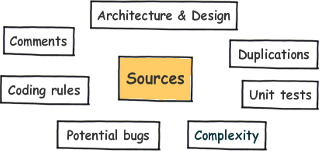
\includegraphics[width=0.7\textwidth]{sonar7axes.png}
\caption{Sonar covers 7 axes}
\label{sonar7axes}
\end{figure}

\par This Software gives you the opportunity to integrate with your Source code management and a result metrics result visualization panel with Nemo - \url{http://nemo.sonarsource.org/} using Saas solution through \emph{Cloud Bees} - \url{http://www.cloudbees.com/platform-service-sonarsource.cb}.

\begin{figure}[H]
\centering
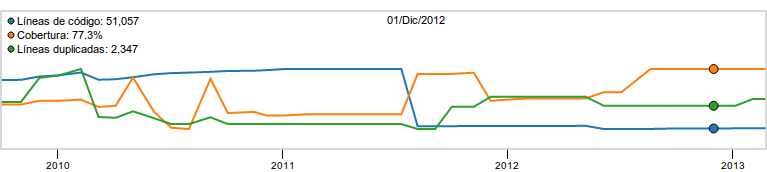
\includegraphics[width=0.7\textwidth]{nemo-evolution.png}
\caption{}
\label{}
\end{figure}

\par Sonar is focused in code Analysis its market niche as Code Climate but offering easy configurable solutions for integrate your projects with giving you the possibility to analyze our software and visualize the results among time.

\par This is our niche, Software Analysis, visualization and interoperability between Source Code Management.

% subsection sonar (end)
% section market-niche (end)

\section{Management general path}
\label{sec:management-path}

\par services and personal.

% section management-path (end)

\section{Management Policies}
\label{sec:management-policies}

\par Communities, Enterprise ROLE, Single Vendor or Apache Software Foundation.

% section management-policies (end)
\subsection{Where will be published the code ?}
\label{sub:publish-code}

\par First is not where, first is, which SVC - \emph{System Version Control} - will be used ?

\par We choose a DVC - \emph{Distributed Version Control} - System instead of an CVC\emph{Centralized Version Control} System. A \emph{DVC} increases the capabilities to developers (including community contributors) to develop solutions and test their development in every environment. The main reason is that a \emph{DVC} gives you the opportunity to work without being connected to internet and save all your historical revisions. The other reason is that applying \emph{DVC} Systems (mainstream) workflow Branch per Feature from Martin Fowler analysis\cite{branch-per-feature} and how to fit with Continuous Integration Development, increases the productivity and facilitates the integration of new developments minimizing the problems with merging in \emph{CVC}s. Thinking about publishing a project as FLOSS with the idea of creating a solid and integrate community we must use a \emph{DVC}.

\par The are different \emph{DVC}s to choose:
\begin{itemize}
    \item Monotone - \url{http://www.monotone.ca/}. monotone is a free distributed version control system. It provides a simple, single-file transactional version store, with fully disconnected operation and an efficient peer-to-peer synchronization protocol. \emph{Introduced hash commits}.
	\item GNU Arch - \url{http://www.gnu.org/software/gnu-arch/}. It is used to keep track of the changes made to a source tree and to help programmers combine and otherwise manipulate changes made by multiple people or at different times.
	\item Bazaar - \url{http://bazaar.canonical.com/en/}. Bazaar is a version control system that helps you track project history over time and to collaborate easily with others. \emph{GNU Arch fork}.
	\item Darcs - \url{http://darcs.net/}. Darcs is a free and open source, cross-platform version control system, like git, mercurial or subversion but with a very different approach. Thanks to its focus on changes rather than snapshots, Darcs can offer a freer way of working, and a simpler user interface. It's written in \emph{haskell}.
	\item Git - \url{http://git-scm.com/}. Git is a free and open source distributed version control system designed to handle everything from small to very large projects with speed and efficiency.
	\item Mercurial - \url{http://mercurial.selenic.com/}. Mercurial is a free, distributed source control management tool. It efficiently handles projects of any size and offers an easy and intuitive. 
\end{itemize}

\par After a deep analysis for choose one \emph{DVCs}. We decided to use Git. Our decision is based in the facility to propagate through internet, most development forges allow and promote the use of Git instead of others, this could be a hype but a hype that works because if this system has not a good \emph{interoperability} APIs and easy hooks configurations will be replaced easily. And was born from Linus Torvalds after BitKeeper affair with taxes and its 'special' license clause\footnote{\url{http://kerneltrap.org/node/444}} to manage Linux kernel source.

\par After choosing Git we must decide where. We decided to host our Git Repository in Github - \url{https://github.com/} - Projects and community in Github have a lot of visibility and i uses a clean user-friendly interface furthermore is a Git powered forge that allows an easy implementation of hooks to our repositories. Why is this important to us ? Because our project is a code analyzer where could be better hosted to be tested than in an easily interoperability configurable forge that spread hook integration. I think this forge increases the visualization to your work, organization capabilities and community communication, the most important issue.

% subsection publish-code (end)

\subsection{Communication strategy and channels}
\label{sub:communication-strategy}

\par In communication staging we have to accomplish with two main groups: \emph{strategy} and \emph{channels}.

\par Starting with \emph{Jono Bacon}\cite{art-of-community} introduction to \emph{Communicating Clearly} chapter:
\begin{quotation}
    \emph{"Community is absolutely about understanding the ether. Our notes are the processes, governance, tools, and methods in which we work together. The notes we don’t play are the subtle nuances in how we pull these notes together and share them with one another. The space between the notes is communication."}
\end{quotation}

\par Stands as the centrepiece of his chapter, the most important thing in communication within a community are \emph{"the notes you do not play"}, citing a quote from Eric Clapton. That is, when we know which is the vehicle we need to introduce for proper communication. It is more important that we miss something than overcharge the channels

\par Therefore, we will divide the process into two phases. Using the analogy of the roads and driving through them we have:
\begin{itemize}
	\item Create the highways - Channels: such as mailing lists, forums, and discussion channels.
    \item Encourage great driving - Strategy: providing a consistent example of simple approaches to communication that make the community easier to understand and more pleasurable for everyone involved)
\end{itemize}

\par Thinking about our project, \emph{Greenhouse} is a technical project for technical users. This is the first step to choose an appropriate channel. We have developers in our company and first users (that could became developers) thus we want to separate the communication between two channels:

\begin{itemize}
	\item Mailing lists: Create different mailing lists for each type of subscriber: developer, user. 
	\item Forums: Forum to get an easy human enter door to the project for a newbie developer and not expecting to be the main communication channel.
\end{itemize}

\subsubsection{Mailing Lists}
\label{sub:mailing-lists}

\par Be clear, specific and human (the most important). In Mailing Lists we have to be in touch with the people interested to contribute to the project, not only the short term upstream, we are focused in long term upstream. Thus we have to be organized, focused and good mates. \emph{Mailing Lists} will be public and this has to be in the whole project, because of transparency we can create a trustful community around the project.

\par Starting with mailing list, we need a clear language, follow Netiquette\footnote{\url{http://tools.ietf.org/html/rfc1855}} basic guidelines and respect everyone’s opinion. 

\par Avoiding the main problems in Mailing List such \emph{bikeshed}\footnote{The gist is that while nobody will question the details of a large and complex project (e.g. a nuclear reactor), for a simple thing as a bikeshed everybody will loudly add their two cents as to exactly how it should be built/painted/constructed} and over technique discussions which can drive away new community members.

\par \emph{Mailing Lists} have to be maintained and guided by the community thus we have to be clear and describe process, guides and documentation.

% subsubsection mailing-lists (end)
\subsubsection{Forums}
\label{sub:forums}

\par The \emph{Forums} create a friendly user interface for a newbie users to get in touch with community and little problems that couldn't fit well in our \emph{Mailing Lists}. Gives the opportunity to search and reply easily. To the new user or the user that only is looking for one determinate question, such as FAQS\footnote{Frequent Ask Questions} or version release posts.

\par \emph{Forums} maintenance could be assumed by a developer (in the beginning) and other forum users that increase its participation and rank by meritocracy inside the \emph{Forum}. The purpose of the forum is to be handled by community to introduce a friendly-human face to newbie users.

% subsubsection forums (end)

\par After chose these \emph{"highways"} and \emph{"Encourage great driving"} we need documentation, clear documentation related to this tools. How to get started and how to choose the right \emph{"highway"}. This will guide the user (pre-community user) into the channels and facilities of community. 

\begin{itemize}
	\item Where are the tools ?
	\item How to start. Firs search, is not necessary to be register to search for information. Transparency and increasing engagement with the community interacting.
	\item Guides and rules to write, showing samples. Friendly and human samples. For the administrator and the basic user.
	\item FAQs - Resolved issues, HowTo's, help and where is.
\end{itemize}

\par Furthermore we have to use blogs, create and produce content related to the community, personal blogs, technical blogs, articles, stories about the community, talks and success cases. This could be another highway to spread information about the community and the project.

\par If you are looking for IRC channel, you won't find it. We started this section referring us to the appointment of Jono Bacon \emph{"the notes you do not play"} therefore we decided not to create an IRC Channel for the community because we can't manage it whit our resources. Ff the community will want one we will be happy and could try to afford this cost in the future.

% subsection communication-strategy (end)

\subsection{Managing volunteers and attracting new users}
\label{sub:volunteers-users}

% subsection volunteers-users (end)

\section{Technology}
\label{sec:technology}

\par Commodity.

% section technology (end)

\subsection{Technical Infrastructure needed}
\label{sub:infrastructure}

\par Rationality, critical analysis, Development plan (good practices for source code development) and roadmap.

% subsection infrastructure (end)

\section{Business scalability}
\label{sec:scalability}

\par Metasploit and MySQL.

% section scalability (end)

\subsection{Evolution}
\label{sub:evolution}

\par Teams, Volunteers, Expansion. Where , How, Which mechanisms ?

% subsection evolution (end)

\subsection{Emphasis}
\label{sub:emphasis}

\par Integration, Upstream.

% subsection emphasis (end)

\begin{thebibliography}{9}

    \bibitem{your-cake}
    Philip H. Albert,\\
    Dual Licensing: Having Your Cake and Eating It Too,\\
    http://www.linuxinsider.com/story/38172.html

    \bibitem{revoking-gpl}
    Milking The GNU,\\
    Dual-licensing: revoking the GPL,\\
    http://blog.milkingthegnu.org/2008/05/dual-licensing.html

    \bibitem{unfair}
    Milking The GNU,\\
    Dual-licensing is unfair and community debilitating,\\
    http://blog.milkingthegnu.org/2008/05/exisiting-dual.html

    \bibitem{mit-gpl}
    StackOverflow,\\
    MIT GPL Dual-license in commercial software,\\
    http://stackoverflow.com/questions/3336161/mit-gpl-dual-license-in-commercial-software

    \bibitem{dual-license-schemes}
    Producing OSS,\\
    Dual Licensing Schemes,\\
    http://producingoss.com/en/dual-licensing.html

    \bibitem{dl-business-model}
    Elena Blanco,\\
    Dual-Licensing As A Business Model,\\
    http://www.oss-watch.ac.uk/resources/duallicence2

    \bibitem{brian-behlendorf-business-strategy}
    Brian Behlendorf,\\
    Open Source as a Business Strategy,\\
    http://oreilly.com/openbook/opensources/book/brian.html
    
    \bibitem{branch-per-feature}
    Martin Fowler,\\
    FeatureBranch,\\
    http://martinfowler.com/bliki/FeatureBranch.html
    
    \bibitem{art-of-community}
    Jono Bacon,\\
    The Art of Community,\\
    http://www.artofcommunityonline.org/
\end{thebibliography}

\end{document}
